\section{Case Studies}
\label{sec:caseStudy}
In order to quantify the effects of optimizing the scripts, we performed a case study.
We say that a C\# method is {\em intrinsicable} if it is a .NET Framework method for which the SCOPE compiler has a semantically equivalent C++ function.
The jobs were chosen based on a static analysis that found {\em optimizable vertices}.
An optimizable vertex is one that is implemented in C\#, but the C\# code calls only intrinsicable methods or user-defined functions, {\em UDFs}, where the UDF, in turn, calls only intrinsicable methods, and does not call any other UDFs, i.e., our inlining depth is one.
Furthermore, we identified a job as being of interest if it contains an optimizable vertex was responsible for X\% of the total job's time.
{\bf mb:[Marija, is that true? Or did we just care about the cost of the job?]}
We categorized the jobs by how long they ran for: short, medium, and long.
{\bf mb:[Marija, do you have any stats about the distribution of PnHours? Are there really just three buckets? [0,100), [100,1000), and [1000,...)?]}

Because the input data for each job is not available, we needed to contact the job owners and ask them to re-run the job with a manually-inlined version of their script.
We were able to have only a few jobs re-run by their owners.

We illustrate the difference that replacing a C\# vertex with a C++ vertex can make.
Job A is a medium-expensive job that runs daily.
It contains one vertex that had been implemented in  C\# because of a single user-defined function.
Inlining that one function resulted in the entire vertex being executed in C++.
Figure~\ref{fig:CaseStudyA} shows the CPU time for that vertex over an 18 day period, the last 5 of which were with the inlined UDF.
The values are all normalized by the average of the unoptimized execution times; the optimized version saves approximately 60\% of the execution time.

\begin{figure}[ht]
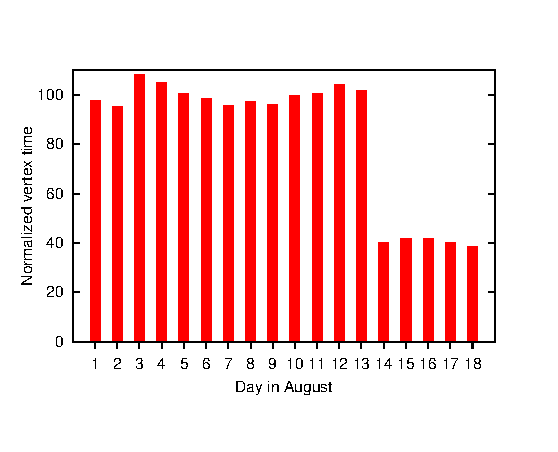
\includegraphics{graphs/normalizedTimes}
\caption{Case Study A \label{fig:CaseStudyA}}
\end{figure}

We looked at 3 other jobs, summarized in Figure~\ref{fig:caseStudySummary}.
One of them turned out to be a false positive, where we mistakenly thought a method was an intrinsic.
For the other two, we were not able to perform the same kind of historical study: instead we have just one execution of the optimized script.
\begin{figure}[ht]
\begin{tabular}{c|c|c|c|c|c} 
{\em Job Guid} & {\em Vertex} & {\em Job Name} & {\em Job Cost} & {\em Vertex Improvement} & {\em Job Improvement} \\ \hline
01e72a39 & SV4\_Extract & B & low & 41.98\% & 25.00\% \\
0414cd51 & & C & false positive \\
f2bd0961 & SV1\_Extract\_Combine\_Split & D & high & 7.22\% & 4.79\%
\end{tabular}
\caption{Summary of case studies. {\sc Delete the job guid and vertex columns before submitting!}
\label{fig:caseStudySummary}}
\end{figure}




\begin{itemize}
\item Description of every optimized job
\item Performance evaluation (methodology)
\item At least one job that changes algebra
\item At least one job that does not change algebra
\end{itemize}
